% !TeX spellcheck = it_IT
%Carattere dimensione 12
\documentclass[12pt]{report}

%Margini e interlinea
% \linespread{1.5}

%Librerie utili
\usepackage[italian]{babel} % conversione in italiano

\usepackage{libertine}
\usepackage{graphicx}
\usepackage{amsmath}
\usepackage{pgfplots}
\usepackage{amssymb}
\usepackage{bm} % fornisce il comando \bm per il testo in grassetto
\usepackage[utf8]{inputenc}
\usepackage{float} % aggiunge l'opzione H alle "floating figures"

% \usepackage[strict]{changepage}
% \usepackage{floatflt}
% \usepackage{blindtext}
% \usepackage{enumitem}
% \usepackage{amsthm}
% \usepackage{subfig}
% \usepackage{listings}
% \usepackage{listingsutf8}
% \usepackage{framed}
% \usepackage{minibox}
% \usepackage{wrapfig}
% \usepackage{longtable}

\usepackage{standalone}
\usepackage{tikz}
% \usepackage{csquotes}


\pgfplotsset{width=11cm,compat=1.9}
\usepgfplotslibrary{external}
\usetikzlibrary{external}
\usetikzlibrary{positioning}
\usetikzlibrary{arrows}
\usetikzlibrary{calc}
\tikzexternalize


\usepackage[top=3cm, bottom=3cm, left=3cm, right=3cm]{geometry}
\pagestyle{plain}
\linespread{1.5}

\usepackage[backend=biber]{biblatex}
\addbibresource{references.bib}

% \definecolor{funcolor}{HTML}{ef8a62} %TODO: externalize styles
\definecolor{funcolor}{HTML}{427ef5} %TODO: externalize styles

\begin{document}

\begin{titlepage}
  \begin{figure}[t]
    %\centering
\includegraphics[width=0.9\textwidth]{marchio-unipi.eps}
    \centering
\includegraphics[width=0.9\textwidth]{./img/logo.eps}
    
    \vspace{1cm}
    
    \centering
\includegraphics[width=0.4\textwidth]{./img/cherubino.eps}
  \end{figure}

  \begin{center}
    \textbf{ Dipartimento di Informatica\\ Corso di Laurea Triennale in Informatica\\}
    \vspace{15mm}
    {\LARGE{\bf Localizzazione Indoor Basata su Beacon Bluetooth a Bassa Potenza
    Attraverso Tecniche di Deep Learning}}\\
    % \vspace{3mm}
    % {\LARGE{\bf Attraverso Tecniche di Deep Learning}}\\
    {\large{\bf un progetto realizzato per Consorzio Metis e ASL Toscana}} \\
  \end{center}

  \vspace{20mm}

  \begin{minipage}[t]{0.47\textwidth}
    {\large{\bf Relatori:\\ Prof. GianLuigi Ferrari 
    % \\ Prof. Alessio Micheli
    }}
  \end{minipage}\hfill
  \begin{minipage}[t]{0.47\textwidth}\raggedleft
    {\large{\bf Presentata da: \\ Marco Pampaloni}}
  \end{minipage}

  \vfill


  \centering{\large{\bf Anno Accademico 2019/2020 }}

\end{titlepage}



\begin{abstract}
  % \begin{figure}
  %   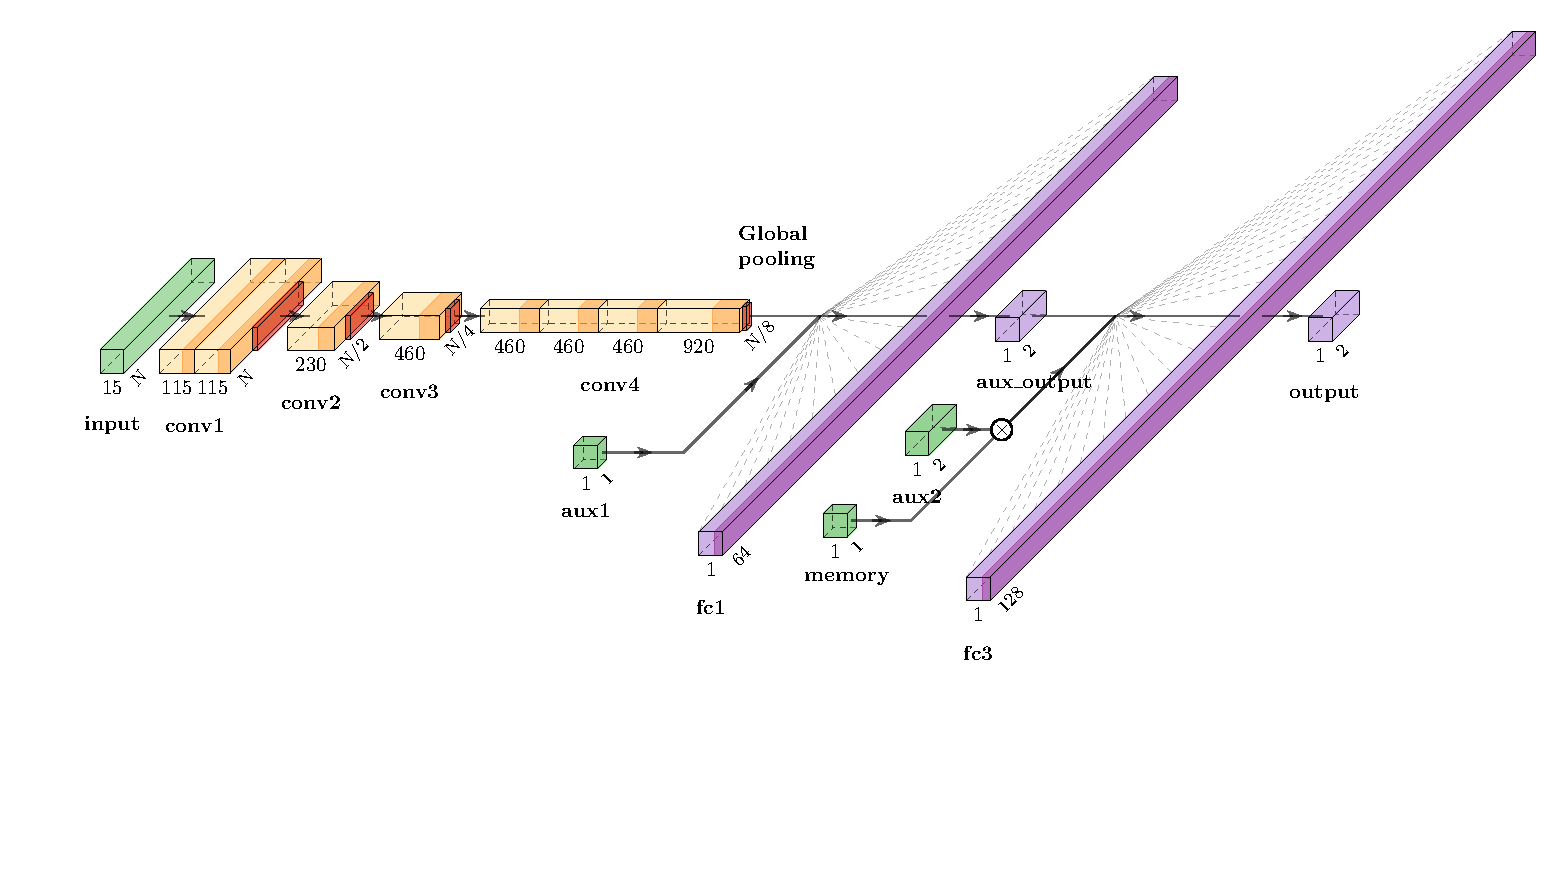
\includegraphics[width=\textwidth]{./img/architettura.pdf}
  %   \caption{Architettura Neurale}
  % \end{figure}
  \documentclass{standalone} 
\begin{document}
% \section{Background}
Il problema della Localizzazione Indoor si è rivelato di particolare interesse
pratico negli ultimi anni. Questa tesi mostra come moderne tecniche di Deep
Learning possano risultare determinanti nella corretta risoluzione di tale
problema.
\\
% \section{Methods}
L'approccio analizzato sfrutta una rete neurale convoluzionale (CNN) profonda:
l'input del modello è caratterizzato da una serie temporale di segnali
broadcast \emph{Bluetooth Low Energy} (BLE) emessi da un insieme di Beacon
disposti all'interno dell'edificio adibito alla Localizzazione Indoor, mentre
l'output è una coppia di coordinate relative alla posizione all'interno
dell'edificio stesso. Sono state inoltre utilizzate varie tecniche di
\emph{data augmentation} per produrre un dataset di grandi dimensioni sulla
base dei campionamenti dei segnali effettuati in loco.
\\
% \section{Results}
A seguito dell'addestramento, il modello utilizzato ha mostrato un errore medio
assoluto (MAE) sul dataset di test pari a \emph{30cm}, esibendo una discreta
affidabilità anche rispetto a variazioni significative dei segnali dovute al
rumore ambientale. Un ensemble di modelli, ognuno addestrato con diversi
iperparametri, ha permesso di ridurre l'errore medio fino a circa \emph{26cm}.
\\
Il modello prodotto risulta eseguibile in tempo reale su dispositivi
mobile con ridotte capacità computazionali, rendendolo particolarmente adatto
alla 
% \section{Conclusion}
così detta navigazione \emph{``blue-dot``} all'interno di contesti Indoor.
Tuttavia si evidenzia come la variazione dell'output del modello possa
risultare in una navigazione poco fluida. Per arginare questo problema viene
applicato un filtro di Kalman al modello e viene sfruttato il sensore inerziale
dello smartphone per produrre un'euristica utile a individuare i movimenti
dell'utente.  
\end{document}

\end{abstract}

\tableofcontents

\chapter{Introduzione}
\documentclass[draft]{standalone}
\begin{document}
%Problema
\section{Localizzazione Indoor}
Il problema della Localizzazione Indoor consiste nell'individuazione di un
utente all'interno di uno spazio chiuso, in riferimento a un sistema di
coordinate predefinito. Tale sistema di coordinate, relativo ad un determinato
edificio, può essere poi espresso in termini georeferenziali conoscendo la
precisa dislocazione geografica del locale in questione. 

La localizzazione indoor apre le porte a diverse possibilità nel campo
dell'esperienza utente all'interno di edifici pubblici, nel settore della
gestione dei flussi di persone, della sicurezza e della contingentazione. Tali
problematiche si fanno ancora più rilevanti a fronte della recente epidemia di
Covid-19 che ha colpito il pianeta. Attraverso l'impiego di tale tecnologia è
possibile coadiuvare la navigazione degli utenti all'interno di edifici
complessi, assicurare il rispetto delle norme di distanziamento sociale
interpersonale e migliorare l'esperienza individuale di persone affette da
disabilità. Per ottenere questi risultati è però richiesto un certo grado di
precisione, di affidabilità, di efficienza e di sicurezza nella gestione della
privacy dei dati di localizzazione degli utenti. Inoltre la tecnologia scelta
per risolvere il problema, per essere fruibile, deve avere come ulteriore
requisito il basso impatto economico.

\section{Soluzioni Tecnologiche}
%Letteratura
Nel corso degli anni sono state implementati diversi sistemi di localizzazione
indoor, che possiamo dividere in due macrocategorie: soluzioni ad-hoc e
soluzioni che sfruttano tecnologie esistenti. Nel primo caso si fornisce
all'utente l'attrezzatura necessaria ad essere localizzato, mentre nel secondo
si utilizza un dispositivo mobile di proprietà dell'utilizzatore.  Spesso tale
dispositivo è uno smartphone. 

I sistemi che implementano tecnologie sviluppate ad-hoc, sono spesso più
efficienti, più precisi e flessibili. Tuttavia, il loro impiego rimane limitato
a causa dell'alto costo di progettazione, installazione e di gestione. È poi
richiesto che ad ogni utente che intenda essere localizzato sia assegnato un
dispositivo che si interfacci col sistema impiegato.

Per l'impiego su larga scala, un sistema di localizzazione indoor deve essere
facilmente utilizzabile dalle masse e non deve richiedere particolari requisiti
tecnologici.

\section{Bluetooth Low Energy}
La tecnologia \emph{Bluetooth} è talmente pervasiva che ogni smartphone in
circolazione ne implementa il protocollo, mostrandosi particolarmente adeguata
alla risoluzione del problema in esame. Nello specifico, \emph{Bluetooth Low
  Energy} (BLE) è un protocollo che riduce notevolmente il consumo energetico
dei dispositivi che lo utilizzano. La tecnologia BLE viene utilizzata dalle
moderne API di \emph{contact tracing} sviluppate da Apple e Google, nonchè
dalla applicazione Immuni\cite{immuni} per il tracciamento dei contagi di
Covid-19\cite{apple-google}.

La soluzione riportata in questo elaborato prevede l'utilizzo di una serie di
beacon BLE programmabili, ciascuno installato in un punto significativo
dell'edificio e configurato per emettere un segnale broadcast con una frequenza
di circa 50Hz. La potenza dei segnali viene quindi utilizzata per produrre,
attraverso l'utilizzo di una rete neurale artificiale, una coppia di coordinate
rappresentative della posizione dell'utente all'interno dell'edificio. Ciò
viene reso possibile da una fase preliminare in cui viene mappata la superficie
del locale raccogliendo i segnali ricevuti dai beacon in vari punti. Per ogni
punto della superficie mappato si registra una serie temporale di segnali, dei
quali si considera solo il valore \emph{RSSI}, ovvero la potenza del segnale
nel punto in cui questo viene ricevuto.

Il modello utilizzato è di fatto completamente agnostico rispetto
all'ubicazione dei beacon installati, supponendo che questa sia unica e non
mutabile nel tempo.

L'utilizzo di tale sistema assicura il completo anonimato dell'utente, il quale
non necessita di condividere la propria posizione, essendo quest'ultima
calcolata direttamente sul suo smartphone in funzione dei segnali che riceve.

% Contenuto
Questo elaborato si pone l'obiettivo di descrivere nello specifico la rete
neurale progettata per risolvere il problema, le tecniche utilizzate per alzare
il grado di precisione del modello e le principali differenze rispetto a
modelli già esistenti.

% \section{Installazione dei Beacon e Acquisizione dei Dati}

\end{document}

\section{RSSI e propagazione del segnale}
\section{Variabilità e rumore di fondo: requisiti di usabilità}
\section{Installazione dei Beacon e Acquisizione dei Dati}

\chapter{Deep Learning}
\documentclass{standalone}

\begin{document}
In questo capitolo saranno introdotti i concetti fondamentali alla base delle
moderne tecniche di Deep Learning e le strutture matematiche necessarie alla
loro comprensione. \\

\section{Machine Learning}
Il \emph{Machine Learning}, o apprendimento automatico, è un insieme di
tecniche e algoritmi che consente a dei programmi di ``imparare'' a svolgere
un determinato compito sulla base di esperienze pregresse, senza bisogno da
parte del programmatore di specificare come eseguire tali mansioni. 
\subsection{Regressione Lineare}
Un classico esempio di algoritmo di machine learning è quello della regressione
lineare. Scopo dell'algoritmo è predire l'output di una determinata funzione.
Si consideri quindi un vettore $ \bm x \in \mathbb{R}^n $, e un valore scalare
$\hat{y} = \bm \theta^\intercal \bm x$. il vettore $\bm \theta$ introduce i
parametri del modello, mentre $\hat{y}$ ne rappresenta l'output, che è una
funzione lineare di $\bm x$. Siano quindi $ \bm x_1, \bm x_2, \dotsc, \bm x_m $
dei vettori in $\mathbb{R}^n$ e  $ y_1, y_2, \dotsc, y_m $ i corrispettivi
valori della funzione $f(\bm x_i)$ che stiamo cercando di approssimare.

Perchè la funzione $\hat{y}(\bm x)$ approssimi $f(\bm x)$ è necessario che i
parametri $\bm \theta$ del modello si adattino in modo da minimizzare la differenza
tra l'output prodotto dal modello e la cosiddetta \emph{ground truth}: $y =
f(\bm x)$. A questo scopo si definisce una metrica di errore propria del
processo di apprendimento: l'errore quadratico medio (MSE dall'inglese) 
\begin{equation} \label{eq:mse}
  MSE = \frac{1}{m} \sum_{i=1}^m{(\hat{y} - y_i)^2} 
\end{equation}

Per minimizzare l'errore sul nostro dataset di test è sufficiente porre a zero
la derivata, rispetto a $\bm \theta$, della nostra funzione di costo. Nel caso
della regressione lineare è possibile risolvere l'equazione risultante
ottenendo un sistema di equazioni che prende il nome di 
\emph{normal equations}.
Esistono tuttavia metodi numerici iterativi che si basano sulle informazioni
fornite dal gradiente della funzione di costo che permettono di aggiornare i
parametri del modello cercando di ridurne l'errore, anche nel caso di modelli
non lineari. L'algoritmo su cui si basano molti dei moderni metodi di
apprendimento del Deep Learning è il \emph{gradient descent} o metodo del
gradiente.

Il metodo del gradiente aggiorna i parametri $\bm \theta$ del modello secondo
la seguente regola: 
\begin{equation} \label{eq:grad-up}
  \bm \theta' = \bm \theta - \eta \nabla_{\bm \theta} J(\bm \theta) 
\end{equation}
dove $J(\bm \theta)$ rappresenta la funzione di costo associata al modello,
mentre $\eta$ è un coefficiente chiamato \emph{learning rate}.
%Intuizione gradient descent
Un'interpretazione dell'algoritmo è data dalle informazioni sulla monotonia
ottenute dal gradiente della funzione di costo: per $\eta$ abbastanza piccolo
risulta $J(\bm \theta') \leq J(\bm \theta)$ poichè il gradiente negativo di $J$
determina la direzione di massima decrescita della funzione\cite{goodfellow}.
Ne consegue che applicando ricorsivamente la regola di aggiornamento del metodo
del gradiente, la nostra funzione $\hat{y}$ tenderà ad avvicinarsi alla
funzione originale $y$, minimizzando la funzione di costo.
Possiamo intepretare il coefficiente $\eta$ come la velocità con cui seguire la
pendenza della funzione di errore. \\
{\large TODO: Inserire un'immagine che fornisca un'intuizione del
  funzionamento del gradient descent}

%Gradient descent con MSE e modello lineare
Nel caso di un modello di regressione lineare che usa l'MSE come funzione di
costo, risulta: 
\begin{align*}
  & \forall j \in {1, \dotsc, n}: \\
  \frac{\partial}{\partial\theta_j} MSE &= 
  \frac{\partial}{\partial\theta_j} \frac{1}{m} \sum_{i=1}^m{(\hat{y}_i -
    y_i)^2} \\ 
  %
  &= \frac{\partial}{\partial\theta_j} \frac{1}{m}
  \sum_{i=1}^m{(\bm \theta^\intercal \bm x_i - y_i)^2} \\
  %
  &= \frac{1}{m}
  \sum_{i=1}^m{\frac{\partial}{\partial\theta_j}(\bm \theta^\intercal \bm x_i -
    y_i)^2} \\
  %
  &= \frac{2}{m}
  \sum_{i=1}^m{(\bm \theta^\intercal \bm x_i - y_i)x_i^{(j)}}
\end{align*}
%
Ovvero abbiamo che la regola di aggiornamento è:
$$ \theta'_j = \theta_j - \eta \frac{\partial}{\partial\theta_j} J(\bm \theta)
             = \theta_j - \eta (\frac{2}{m} 
             \sum_{i=1}^m{(\bm \theta^\intercal \bm x_i - y_i)x_i^{(j)}}),
             \quad \forall j \in \{1, \dotsc, n\}
$$

\section{Perceptron}
Il \emph{Perceptron} è il modello che ha posto le basi per le moderne reti
neurali artificiali e il deep learning. Esso prende spunto dalla neurologia,
cercando di imitare il comportamento dei neuroni del cervello umano, con ovvie
limitazioni e senza presunzione di volerne fornire una simulazione accurata del
funzionamento. Una schematizzazione del modello è descritta in Figura
\ref{fig:perceptron}
\def\nodesize{1.0cm}
\tikzstyle{neuron}=[circle, draw=black, minimum size=\nodesize]
\tikzstyle{dots}=[draw=none, scale=2, text height=0.333cm, execute at end node=$\vdots$]
\centering
\begin{tikzpicture}[x=1.5cm, y=1.5cm, >=stealth] % >=stealth arrow style
  % input nodes
  \foreach \m [count=\y] in {1,2,3,dots,n} 
  {
    \ifnum\y=4
    \node [\m/.try] at (0,-\y) {};
    \else
    \node [neuron] (input-\m) at (0,-\y) {$x_\m$};
    \fi
  }
  % middle node
  \node [neuron] (middle) at (1.5, -3) {\LARGE $\Sigma$};

  % activation function
  \node [neuron] (activation) at (3.0, -3) {$g$};

  % connections
  \foreach \m [count=\y] in {1,2,3,n}
  % above moves the text higher depending on the orientation of the line
  \draw [thick, ->] (input-\m) -- (middle) 
  node[above=4pt*abs(3 - \y), pos=0.45, scale=0.9] {$\theta_\m$};

  % middle point between (middle) and (activation) nodes
  \path [thick, ->, draw] (middle) -- (activation) coordinate[pos=0.5] (activation-path);


  % draw sigmoid symbol betwwen (middle) and (activation)
  \draw [thick, scale=0.3, color=funcolor, x=5, y=70, 
  domain=-6:6, yrange=-1:1, 
  shift={($ (activation-path) - (0, 0.5) $) }] % calc library 
  plot (\x, {1/(exp(-\x)+1)});

  % alternative representation of the sigmoid symbol using an integral
  % \draw [thick, ->] (middle) -- (activation) node[midway, above] {
  %   $\displaystyle \int$
  % };

\end{tikzpicture}


Il perceptron è molto simile al modello di regressione lineare descritto
precedentemente, ma si distingue per un fattore fondamentale: la non linearità.
L'output del perceptron è infatti definito come:
$$\hat{y}(\bm x) = g(\bm \theta^\intercal \bm x)$$
dove $g$ è una funzione non lineare che, in questo caso, è una funzione
\emph{sigmoidea}, cioè una funzione che ha un andamento a ``S'', con due
asintoti orizzontali come in Figura \ref{fig:sigmoid}: di solito è utilizzata
la funzione $\displaystyle g(x) = \frac{1}{1 + e^{-x}}$.

Malgrado la nonlinearità del modello, il perceptron non è in grado di
approssimare molte classi di funzioni. È famoso l'esempio della funzione XOR,
la quale non può essere imparata dal perceptron. Per questo motivo è stata
sviluppata un'estensione del modello che prende il nome di \emph{Multi Layer
  Perceptron}.

\begin{figure}[!htp] % place it here (h)
  \centering
  \begin{tikzpicture}
    \begin{axis}[
      grid=both,
      grid style={line width=.1pt, draw=gray!30},
      xlabel=$x$, ylabel={$g(x)$}
      ]
      \addplot[very thick, color=funcolor]{1/(1 + exp(x)^(-1))};
    \end{axis}
  \end{tikzpicture}
  \caption{Funzione sigmoidea $\displaystyle g(x) = \frac{1}{1 + e^{-x}}$ }
  \label{fig:sigmoid}
\end{figure}


\end{document}



\section{Reti Neurali Convoluzionali}
\section{Regolarizzazione}
\subsection{Overfitting e Underfitting}
\subsection{Regolarizzazione L2}
\subsection{Dropout}
\section{Dataset Augmentation e Preprocessing}
\subsection{Jittering}
\subsection{Ridimensionamento (Scaling)}
\subsection{Magnitude Warping}
\subsection{Permutazione di Sottoinsiemi (Subset Shuffling)}
\subsection{Deattivazione Selettiva}


\chapter{Architettura Software}
\section{TensorFlow}
\section{Keras}
\section{Google Colab}
\section{Weights \& Biases}
\section{Modello di Apprendimento}
\subsection{Input del Modello}
\subsection{Blocco Convoluzionale}
\subsection{Uso della Bussola e Output Ausiliario}
\subsection{Coefficiente di Memoria Residua e Input Ausiliario}
\subsection{Output del Modello}
\section{Addestramento del Modello}
\section{Ensembling}
\section{Compilazione e Deploy del Modello}

\chapter{Applicazione Mobile}
\section{Flutter}
\section{Planimetrie e Poligoni}
\section{Backend TensorFlow}
\subsection{TensorFlow Lite}
\subsection{Implementazione del Bridge di Comunicazione}
\section{Stabilizzazione del Modello}
\subsection{Utilizzo di Sensori Inerziali}
\subsection{Filtro di Kalman}

\chapter{Conclusioni}
\section{Risultati Sperimentali}
\subsection{Metriche di Errore: MSE, MAE, MaxAE}

\section{Lavori futuri}
\subsection{Input a Lunghezza Variabile}
\subsection{Reti Neurali Residuali}
\subsection{Variational Autoencoder: Generazione di nuovi dati}
\subsection{Transfer Learning}
\subsection{Input Masking e Ricostruzione dei Segnali}
\subsection{Transformers per Problemi di Regressione}
\subsection{Simulatore BLE}
\subsection{Posizionamento Magnetico}

\appendix

\printbibliography

\end{document}
